%%%%%%%%%%%%%%%%%%%%%%%%%%%%%%%%%%%%%%%%%%%%%%%%%%%%%%%%%%%%%%%%%%%%%%%%%%%%%%%%
% LaTeX Template for UEx - EII documents
% José Emilio Traver Becerra & David Palomeque Mangut
% Use at your own risk, send complaints to {jotraverb,dpalomeq}@alumnos.unex.es
%%%%%%%%%%%%%%%%%%%%%%%%%%%%%%%%%%%%%%%%%%%%%%%%%%%%%%%%%%%%%%%%%%%%%%%%%%%%%%%%

\documentclass[a4paper,openright,titlepage,12pt]{article}

% --------------------------
% Información del documentos
% --------------------------
\newcommand{\myTitle}{ANÁLISIS Y CÁLCULO DE LA VELOCIDAD DE AVANCE GENERADA POR EL MOVIMIENTO DE ONDA VIAJERA MEDIANTE INTEGRACIÓN NUMÉRICA}
\newcommand{\MyTitle}{Análisis y simulación de AFB por \textit{traveling wave}}
\newcommand{\Asignatura}{}
\newcommand{\Degree}{}
\newcommand{\myName}{Nombre Apllido1 Apellido2 (alumno)}
\newcommand{\myProf}{Nombre Apllido1 Apellido2 (tutor1)}
\newcommand{\myOtherProf}{Nombre Apllido1 Apellido2 (tutor2)}
\newcommand{\president}{Nombre Apllido1 Apellido2 (Presidente)}
\newcommand{\vocal}{Nombre Apllido1 Apellido2 (Vocal)}
\newcommand{\secretary}{Nombre Apllido1 Apellido2 (Secretario)}
\newcommand{\myFaculty}{ESCUELA DE INGENIERÍAS INDUSTRIALES}
\newcommand{\myFacultyShort}{E.I.I.}
\newcommand{\myDepartment}{...}
\newcommand{\myUni}{\protect{UNIVERSIDAD DE EXTREMADURA}}
\newcommand{\myLocation}{BADAJOZ}
\newcommand{\myTime}{\MakeUppercase{\today}}
\newcommand{\myVersion}{Version 1.2}


%---------------------------------------
% Paquetes
%---------------------------------------
\usepackage[spanish]{babel}
\usepackage{vmargin}													% Margenes
\usepackage{setspace}
\usepackage{fancyhdr}			   										% Cabeceras
\usepackage[table]{xcolor	}											% Color
\usepackage{color}
\usepackage{multirow}
\usepackage{cite} 														% Para contraer referencias
\usepackage{appendix}												% Para los Anexos.
\usepackage{graphics} 													% Figuras.
\usepackage[justification=centering]{caption}				% Para centrar captions
\usepackage{setspace}													% Modificar el valor del interlineado.
\usepackage[square,sort,comma,numbers]{natbib}		% Bibligrafia	
\usepackage{titlesec}													% Títulos
\usepackage{url}															% URLs
\usepackage[hidelinks]{hyperref} 									% Referencias
\usepackage{enumitem}												% Para enumerar las listas como "X" en vez de "X."
\usepackage{amsmath}													% Entorno matemático.
\usepackage{unicode-math}											% Cambiar fuente de entorno matemático.
\setmathfont{Cambria Math}											% Esta fuente contiene los símbolos.	
%\usepackage{mathastext}											% Fuente en non-italic.
\usepackage{gensymb}
\usepackage{scrextend}
\usepackage{emptypage}   											% Paginas en Blanco
\usepackage{appendix} 												% Anexos
\usepackage{listings}													% Inserter líneas de código
\usepackage[framed,numbered,autolinebreaks,useliterate]{mcode} % Identificación del lenguaje de Matlab y C
\usepackage{listings}

% --------------
% Caligrafía 
% ----------------
\usepackage{fontspec}
%\setmainfont{Calibri}
%\setsansfont{Arial Narrow}

% Letra Charter
%\usepackage[bitstream-charter]{mathdesign} 
\usepackage{textcomp} %Paquete para algunos caracteres especiales

% --------------
% Definir Margenes
% --------------
\setmargins{2cm}       % margen izquierdo
{2.5cm}                % margen superior
{17cm}                      % anchura del texto
{23.43cm}                    % altura del texto
{1.27cm}                           % altura de los encabezados
{0.5cm}                           % espacio entre el texto y los encabezados
{1.27cm}                             % altura del pie de página
{30pt}                           % espacio entre el texto y el pie de página


% ----------------
% Alineación y formato de títulos
% ----------------
\setlength\parindent{0pt}
\setlength{\parskip}{-0.2cm}

\titlespacing\section{0pt}{14pt plus 4pt minus 2pt}{14pt plus 2pt minus 2pt}
\titlespacing\subsection{0pt}{14pt plus 4pt minus 2pt}{14pt plus 2pt minus 2pt}
\titlespacing\subsubsection{0pt}{14pt plus 4pt minus 2pt}{14pt plus 2pt minus 2pt}
\titleformat*{\subsubsection}{\large\bfseries}
\titleformat{\section}{\normalfont\Large\bfseries}{\thesection}{1.8em}{}
\titleformat{\subsection}{\normalfont\large\bfseries}{\thesubsection}{1.5em}{}
\titleformat{\subsubsection}{\normalfont\large\bfseries}{\thesubsubsection}{1em}{}

%--------------
% Tamaños de letras
%--------------
\renewcommand{\small}{\fontsize{10}{12}}					% Small -> 10 pt

% -----------------------
% Cabeceras y Pie de pagina
% -----------------------
\pagestyle{fancy}
\lhead{\fontsize{9}{9} \myTitle \\}
% Modifica el tamaño y la fuente de los pies de página.
\fancyfoot[C]{\thepage \fontsize{9pt}{11pt} }
% Modifica el tamaño de la cabecera (Parte izquierda)
\fancyhead[R]{\scshape \nouppercase{\leftmark} \fontsize{8}{8}}	
\renewcommand{\headrulewidth}{0.4pt} % grosor de la línea de la cabecera
\renewcommand{\footrulewidth}{0.4pt} % grosor de la línea del pie

% --------------------
% Epigrafe Tablas y Figuras
% ---------------------
\captionsetup[figure]{margin=40pt,labelfont={bf,footnotesize},textfont={bf,footnotesize},labelsep=space}
\captionsetup[table]{margin=40pt,labelfont={bf,footnotesize},textfont={bf,footnotesize},labelsep=space}

\renewcommand{\tablename}{Tabla} 											% Cambia la palabra "Cuadro" por "Tabla"
\renewcommand\thefigure{\arabic{section}.\arabic{figure}} 			% Genera numeración X.Y
\renewcommand\thetable{\arabic{section}.\arabic{table}} 			% Genera numeración X.Y

% Numera las Ecuaciones, Figuras y Tablas como X.Y (SECTION.NUMBER)
\numberwithin{figure}{section} 													% Hace que la primera figura de cada sección X sea X.1
\numberwithin{table}{section} 														% Hace que la primera tabla de cada sección X sea X.1
\numberwithin{equation}{section}

% ------------------------
% Nueva Seccion por pagina
% ------------------------
\newcommand{\sectionbreak}{\newpage}

% ----------------------------------------
% Eliminar punto después de la numeración 
% ----------------------------------------
\titlelabel{\thetitle \hspace{10mm}}

% -------------------------------------------
% Subnivel 4º de sección.
% -------------------------------------------
\titleclass{\subsubsubsection}{straight}[\subsection]

\newcounter{subsubsubsection}[subsubsection]
\renewcommand\thesubsubsubsection{\thesubsubsection.\arabic{subsubsubsection}}
\renewcommand\theparagraph{\thesubsubsubsection.\arabic{paragraph}} 
\titleformat{\subsubsubsection}
  {\normalfont\normalsize\bfseries}{\thesubsubsubsection}{1em}{}
\titlespacing*{\subsubsubsection}
{0pt}{3.25ex plus 1ex minus .2ex}{1.5ex plus .2ex}
\makeatletter
\renewcommand\paragraph{\@startsection{paragraph}{5}{\z@}%
  {3.25ex \@plus1ex \@minus.2ex}%
  {-1em}%
  {\normalfont\normalsize\bfseries}}
\renewcommand\subparagraph{\@startsection{subparagraph}{6}{\parindent}%
  {3.25ex \@plus1ex \@minus .2ex}%
  {-1em}%
  {\normalfont\normalsize\bfseries}}
\def\toclevel@subsubsubsection{1}
\def\toclevel@paragraph{5}
\def\toclevel@paragraph{6}
\def\l@subsubsubsection{\@dottedtocline{4}{7em}{4em}}
\def\l@paragraph{\@dottedtocline{5}{10em}{5em}}
\def\l@subparagraph{\@dottedtocline{6}{14em}{6em}}
\makeatother
\setcounter{secnumdepth}{5}
\setcounter{tocdepth}{6}

% --------------------------------
% Márgen izquierdo de la Bibliografía
% --------------------------------
\makeatletter
\renewenvironment{thebibliography}[1]
{\section*{\bibname}%
	\@mkboth{\MakeUppercase\refname}{\MakeUppercase\bibname}%
	\list{\@biblabel{\@arabic\c@enumiv}}%
	{\settowidth\labelwidth{\@biblabel{#1}}%
		\leftmargin\labelsep
		\itemindent1em
		\@openbib@code
		\usecounter{enumiv}%
		\let\p@enumiv\@empty
		\renewcommand\theenumiv{\@arabic\c@enumiv}}%
	\sloppy
	\clubpenalty4000
	\@clubpenalty \clubpenalty
	\widowpenalty4000%
	\sfcode`\.\@m}
{\def\@noitemerr
	{\@latex@warning{Empty `thebibliography' environment}}%
	\endlist}
\makeatother

% ------------
% Anexos
% ------------
\renewcommand{\appendixname}{ANEXOS}			% ANEXOS en vez de Apéndices
\renewcommand{\appendixtocname}{ANEXOS}		%
\renewcommand{\appendixpagename}{ANEXOS}	%

% --------------
% Numeraciones
% --------------
\renewcommand{\labelitemi}{$\bullet$}				% Cambia la muesca en las numeraciones a círculos

%-----------
% Estilo URL
%-----------
\urlstyle{same}																% URLs en Calibri.
\hypersetup{
	colorlinks,
	citecolor=black,
	filecolor=black,
	linkcolor=black,
	urlcolor=blue																% URLs de color azul.
}
	

% --------------
% Colores
% --------------
\definecolor{lightgray}{gray}{0.9}
\definecolor{rosa}{rgb}{1,0.5,0.5}
\definecolor{lbcolor}{rgb}{0.9,0.9,0.9}
\definecolor{Darkgreen}{rgb}{0.0, 0.26, 0.15}
%red, green, blue, yellow, cyan, magenta, black, white


% ---------------------
% Ruta de búsqueda de las figuras
%---------------------
\graphicspath {{Figuras/}}


% -------------------%
% -------------------%
\begin{document}%----%
% -------------------%
% -------------------%

%---------------------------------------
% Portada
%%%%%%%%%%%%%%%%%%%%%%%%%%% Portada.tex %%%%%%%%%%%%%%%%%%%%%%%%%%%%%%%
% Template for producing ---- using LaTeX   						    %
% Written by   Jose Emilio Traver Becerra			                %
% Use at your own risk, send complaints to 		                    %
%%%%%%%%%%%%%%%%%%%%%%%%%%%%%%%%%%%%%%%%%%%%%%%%%%%%%%%%%%%%%%%%%%%%%%

\begin{titlepage}
\begin{center}
\begin{LARGE}
\textbf{Universidad de Extremadura} \\
\end{LARGE}
\ \\
\begin{Large}
Escuela de Ingenierías Industriales\\
\end{Large}
\ \\
\begin{large}
\Asignatura
\end{large}
\end{center}
\vspace{6cm}
\begin{flushright}
%\begin{huge}
\begin{large}
\textbf{\myTitle}
%\end{huge}
\end{large}
\end{flushright}
\vspace{10cm}
\begin{center}
Traver Becerra, José Emilio \\
\Degree
\end{center}
	\begin{center}
		\textbf{\myLocation, \myTime}
	\end{center}
\end{titlepage}



%---------------------------------------



%---------------------------------------
%Tabla de contenidos
%---------------------------------------
\renewcommand{\thepage}{\Roman{page}}		% Numeración en números romanos
\renewcommand{\contentsname}{ÍNDICE}			% INDICE en mayúsculas
\begin{spacing}{1.5}
	\tableofcontents
\end{spacing}
\newpage
\renewcommand{\thepage}{\arabic{page}}		% Numeración en números arábicos
\setcounter{page}{2}											% Contador a cero

%---------------------------------------
% Justificación 
%---------------------------------------
\sloppy 


%--------------- CUERPO DEL DOCUMENTO ----------------

%---------------------------------------
% Capítulo 1: INTRODUCCIÓN 
%---------------------------------------
% Planteamiento del problema
%---------------------------------------
\section{INTRODUCCIÓN} \label{sec:Introduccion}
%---------------------------------------
El presente documento pretender exponer las dificultades algebraicas que plantea el cálculo de la velocidad de avance generada a través del movimiento de onda viajera realizado por microorganismos \cite{Gray1955} y animales acuáticos (peces \textit{Carangiform}) \cite{Korkmaz2012,Korkmaz2011}. Exponer una solución a estas dificultades mediante computación numérica e interpretar y analizar los resultados ofrecidos por la solución propuesta.\\

El movimiento de onda viajera realizado por la mayoría de los peces, según la ictiología es doblando su cuerpo \cite{modeswim}. Este tipo de movimiento denominado \textit{``body and caudal fin''} (BCF) se encuentra categorizado en diferentes clases, de las cuáles el tipo \textit{Carangiform}  presenta la mayor similitud con el flagelo de las células. El movimiento descrito por este tipo de peces fue sugerido originalmente por Lighthill \cite{FLM:368244}, y su expresión matemática es
\begin{eqnarray}
	\label{eq:fish_traveling_wave}
	y (x,t) = (c_1 x + c_2 x^2) \sin \left( \frac{2 \pi}{\lambda}  ( x - V_p t) \right),
\end{eqnarray}
donde $x$ es el desplazamiento sobre el eje principal, $V_p$ la velocidad de propagación de las ondas respecto al cuerpo y de sentido contrario a la velocidad de avance, $\lambda$ la longitud de onda y $c_1$ y $c_2$ los coeficientes lineal y cuadrático de la amplitud de la onda, respectivamente. Esta expresión recoge la dinámica del movimiento \textit{Carangiform} realizado desde el punto de unión del cuerpo hasta el extremo final de la cola \cite{Robotic_Fish,Robotic_Fish_speed,Robotic_Fish_3D}. Para recoger en una misma expresión la posibilidad de una onda viajera armónica como la estudiada para los flagelos en \cite{gray1955propulsion}, se debe introducir un nuevo coeficiente $c_0$ quedando la expresión anterior de la forma
\begin{eqnarray}
	\label{eq:flag_fish_traveling_wave}
	y (x,t) = (c_0+c_1 x + c_2 x^2) \sin \left( \frac{2 \pi}{\lambda}  ( x - V_p t) \right).
\end{eqnarray}

En (\ref{eq:flag_fish_traveling_wave}), el coeficiente $c_0$ permite definir el movimiento armónico puro de la onda viajera, como se ilustra en la Figura \ref{fig:FC}, pero no define el realizado por la cola de un pez. Es necesario sustituirlo por el coeficiente $c_1$, que impone la condición de contorno $y(0,t) = 0$, es decir, el inicio de la cola se encuentra unido a la cabeza en todo instante de tiempo. Sin embargo, dicho coeficiente define una onda viajera cuya amplitud crece linealmente en el eje principal (ver Figura \ref{fig:FC}). Para corregir este comportamiento se introduce el término cuadrático $c_2$, con el cual es posible modular el crecimiento de la onda viajera para alcanzar una amplitud mantenida sobre el eje principal.
\begin{figure}[!h] %  figure placement: here, top, bottom, or page
	\vspace*{3mm}
    \centering
    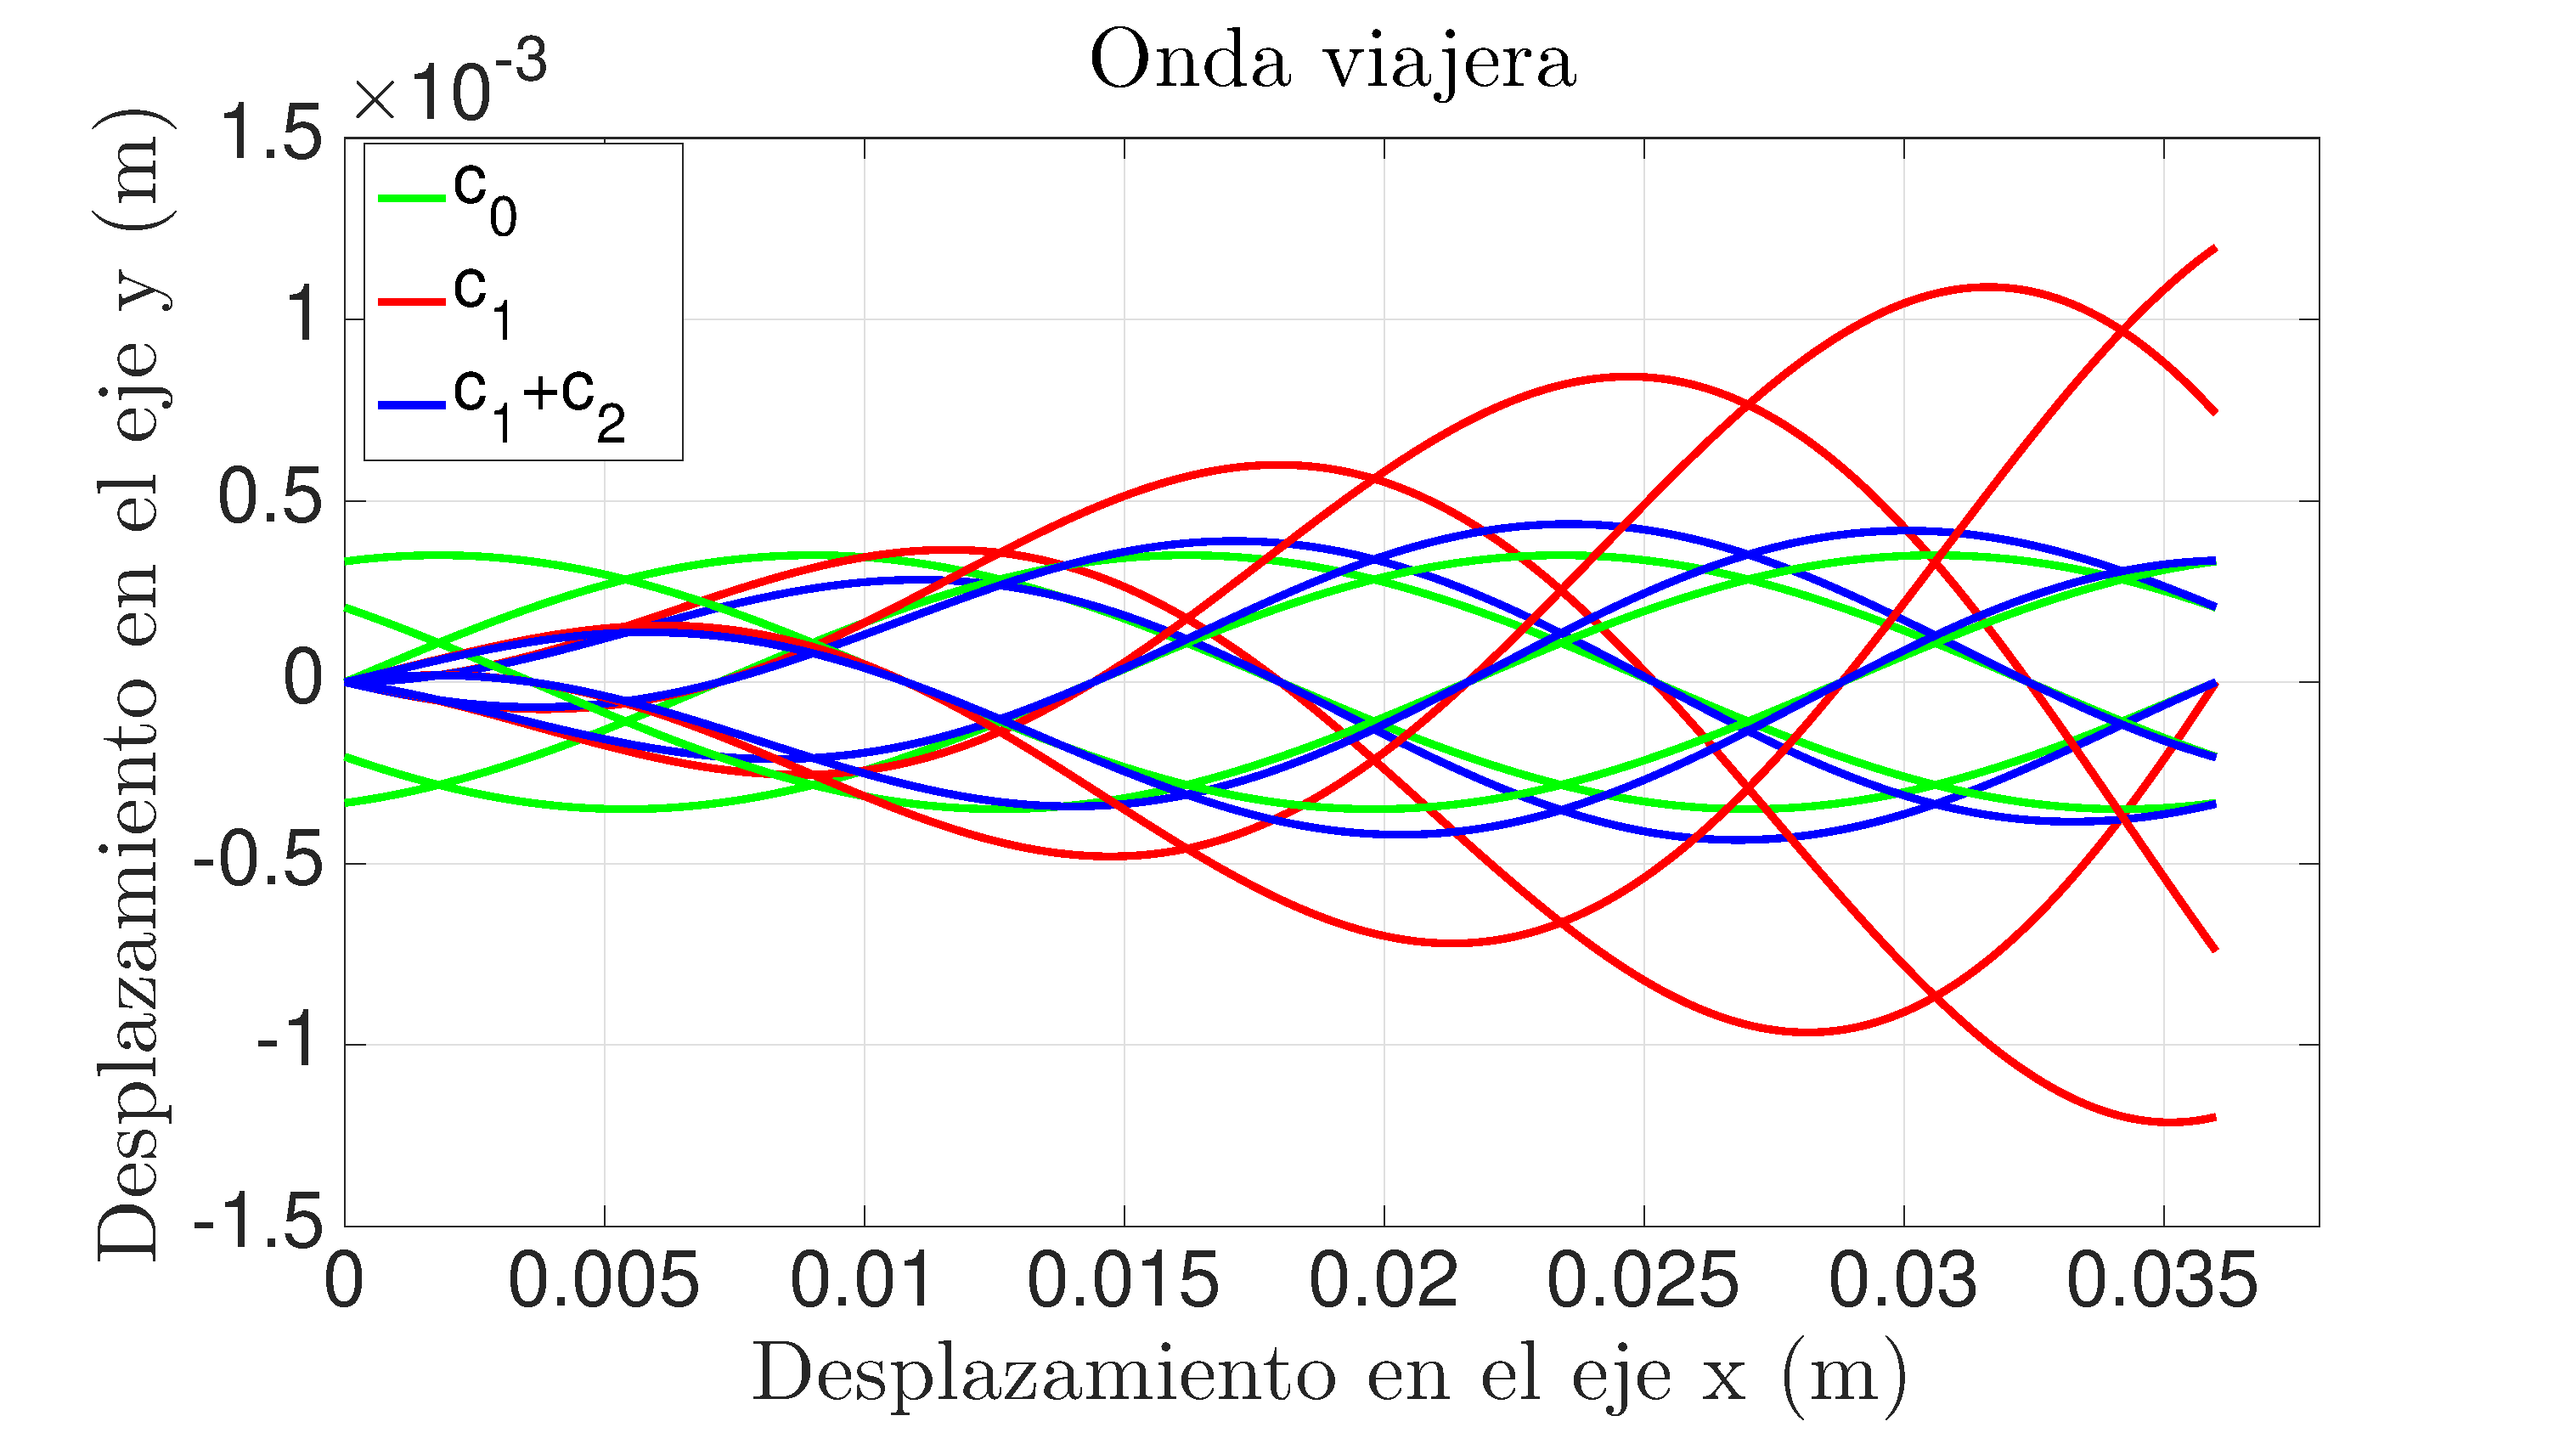
\includegraphics[width=0.43\textwidth]{Figuras/FC}
  	\caption{Comparación de la onda viajera para diferentes coeficientes.}
  	\label{fig:FC}
\end{figure}

Siguiendo el análisis descrito en \cite{gray1955propulsion}, se puede extraer la velocidad de avance para el movimiento indicado en (\ref{eq:flag_fish_traveling_wave}) como:
\begin{eqnarray}
\label{eq:Vx_fish}
\begin{split}
	V_x (t)  =  \pi f\left( \frac{C_N - C_L}{C_L} \right) \left( \frac{1}{ 1 + \frac{6 \pi R \mu}{n \lambda C_L} }  \right)\\
(- \frac{2 \pi}{\lambda} c_0^2 - 2 \pi c_0 c_1 - \frac{4 \pi c_0 c_2}{3} \\ 
+ c_0 c_1 \sin \left( 4 \pi f t \right) + c_0 c_2 \sin \left( 4 \pi f t \right) - \frac{2 \pi \lambda}{3} c_1^2 \\
- \pi \lambda^2 c_1 c_2 + \frac{\lambda c_1^2}{2} \sin \left( 4 \pi f t \right) + \lambda^2 c_1 c_2 \sin \left( 4 \pi f t \right) \\
- \frac{2 \pi \lambda^3}{5} c_2^2 + \frac{\lambda^3 c_2^2}{2} \sin \left( 4 \pi f t \right) )
	 		\end{split}
\end{eqnarray}
donde se aprecia la influencia de los coeficientes para lograr diferentes magnitudes de velocidad, y la relación entre ellos. Esto implica una cierta dificultad para alcanzar una velocidad óptima, y mantener un movimiento de onda viajera cuyas oscilaciones sean moduladas y mantenidas (constantes) en el espacio.\\

Para simplificar este cometido se opta por una descripción diferente del movimiento de onda viajera descrito en (\ref{eq:flag_fish_traveling_wave}), basado en un coeficiente fraccionario que influye en la amplitud de la onda viajera en base a su ubicación en el espacio, siendo por lo tanto la nueva expresión de la forma
\begin{eqnarray}
	\label{eq:flag_fish_traveling_wave_fractional}
	y (x,t) = c_1 x^{\alpha} \sin \left( \frac{2 \pi}{\lambda}  ( x - V_p t) \right).
\end{eqnarray}
\

Esta nueva descripción permite determinar la amplitud máxima de las oscilaciones a partir del coeficiente $c_1$, y modular su crecimiento con el parámetro $\alpha$. La Figura \ref{fig:OVF} evidencia este comportamiento, donde se puede observar el crecimiento en amplitud de la onda para diferentes valores del parámetro $\alpha$.
\begin{figure}[!h] %  figure placement: here, top, bottom, or page
	\vspace*{3mm}
    \centering
    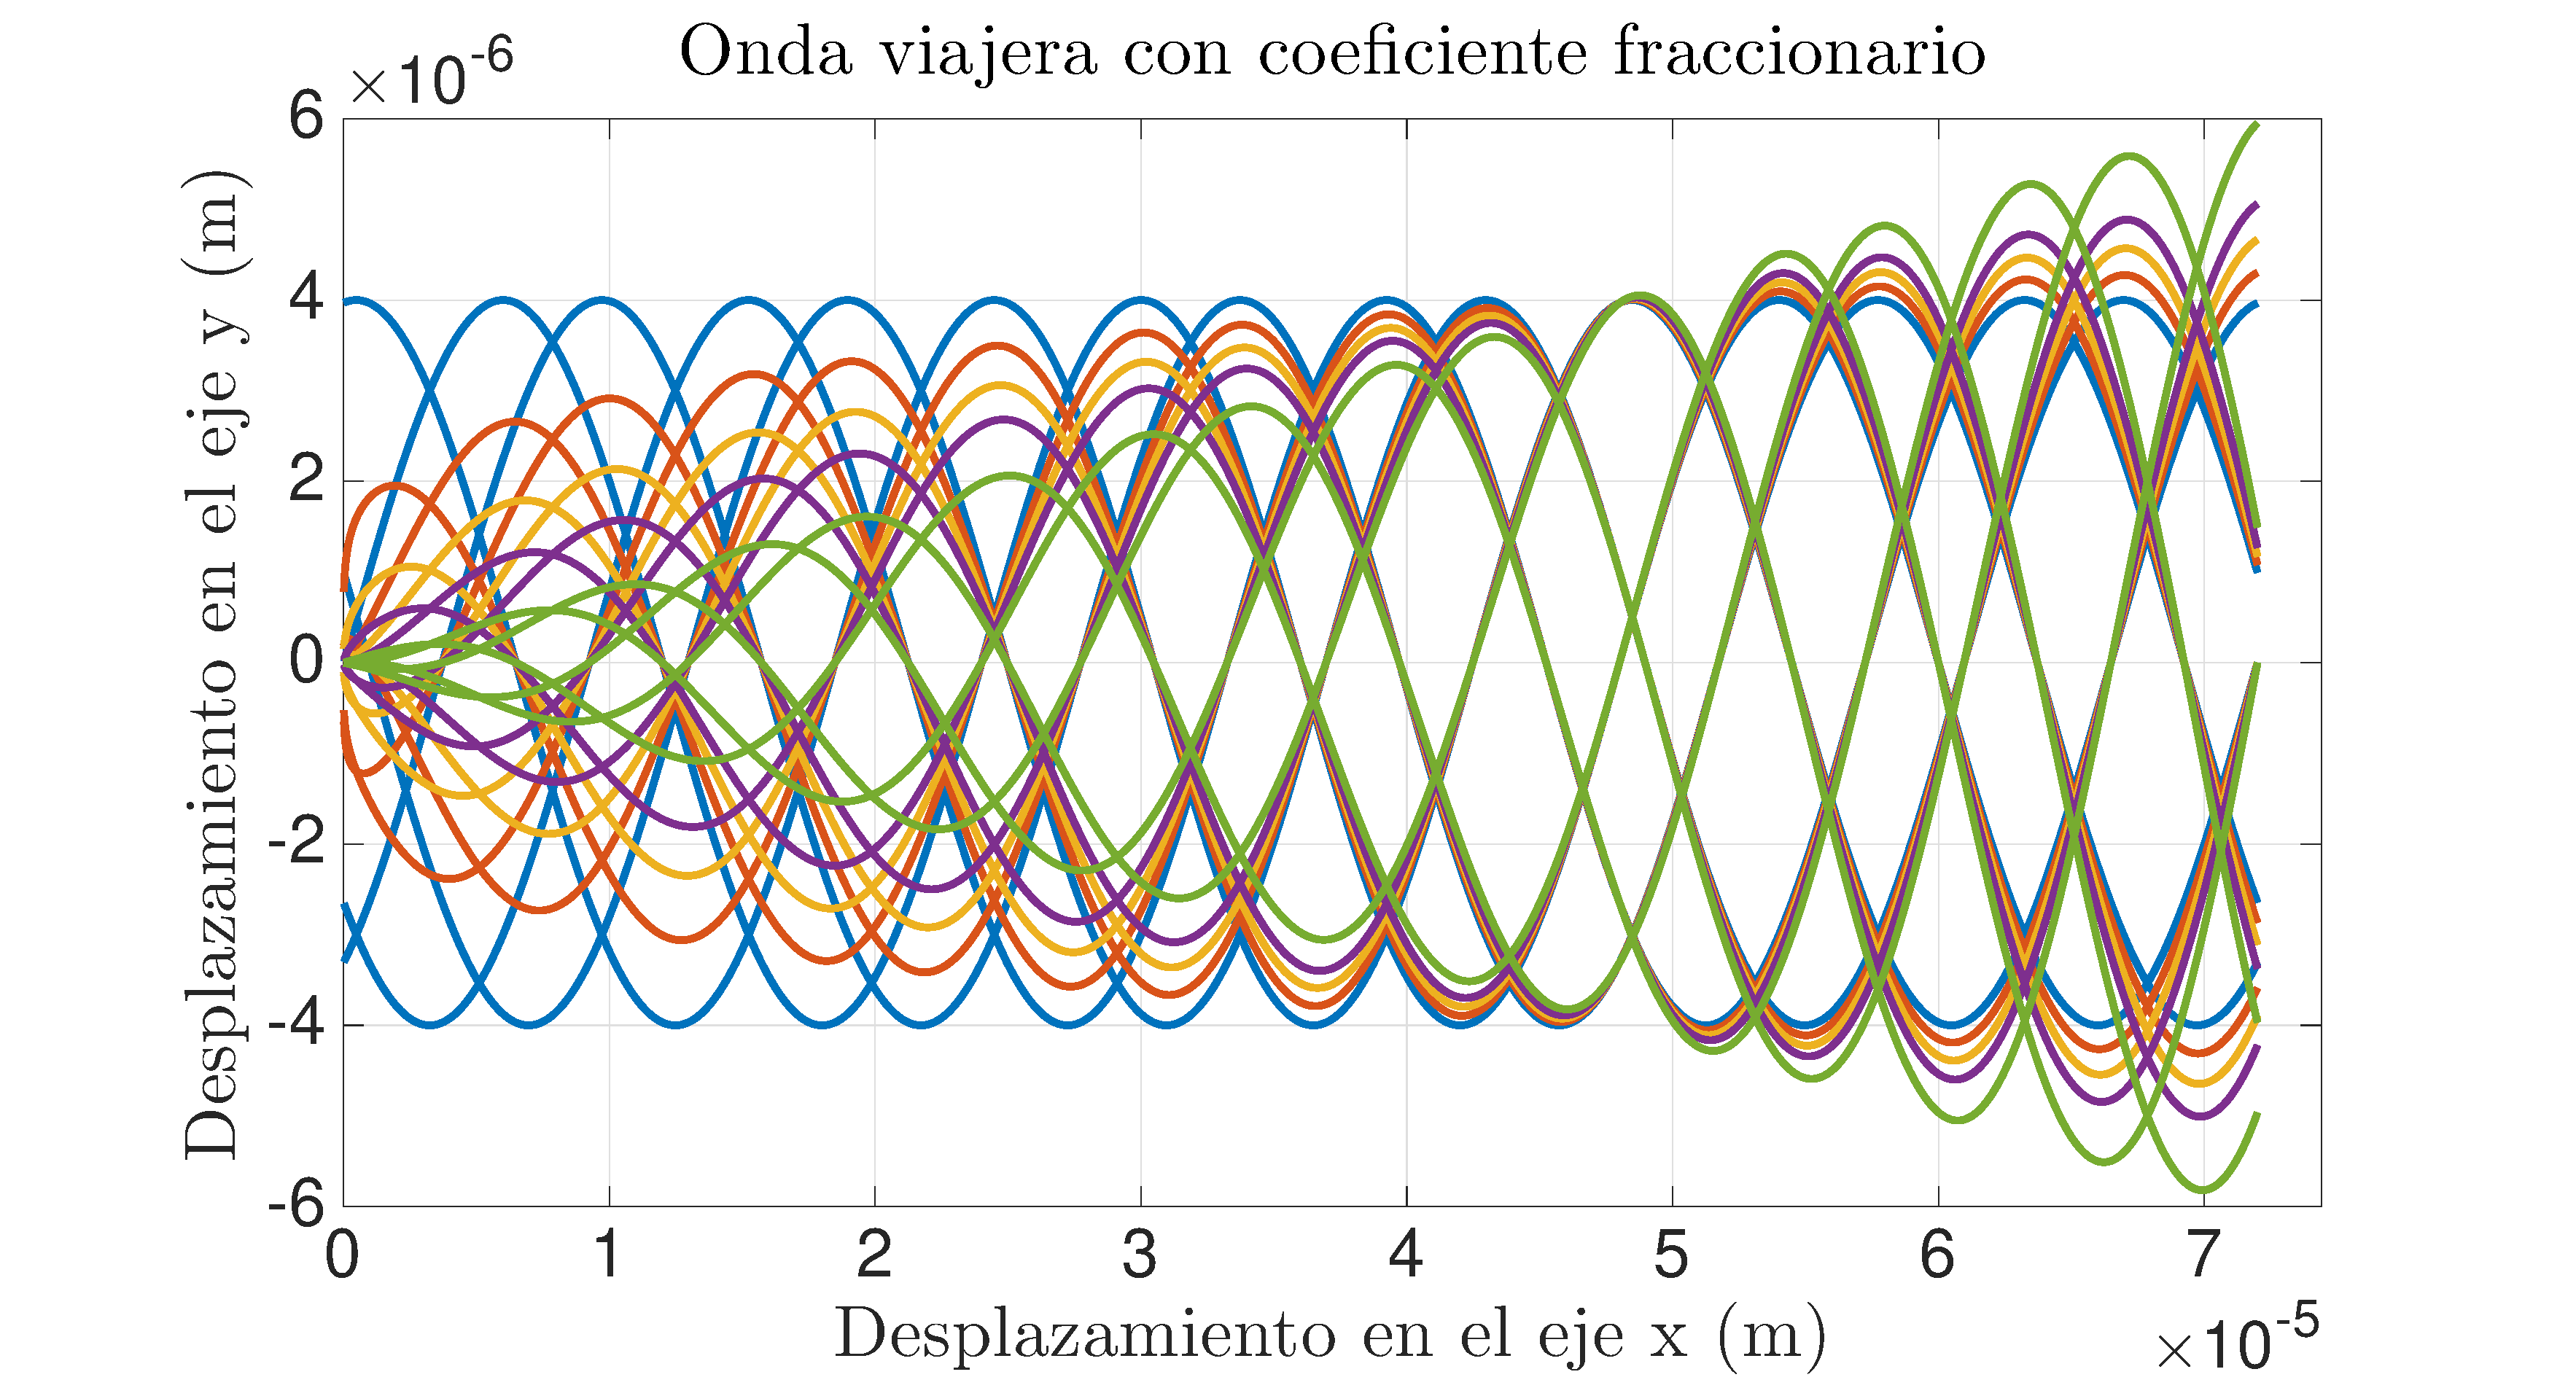
\includegraphics[width=0.6\textwidth]{Figuras/OVF}
  	\caption{Comparación de la onda viajera para diferentes coeficientes fraccionarios.}
  	\label{fig:OVF}
\end{figure}
 En esta representación el coeficiente $c_1$ es definido como $c_1 = \frac{A}{\lambda^{\alpha_0}}$, donde $A$ es la amplitud máxima de la oscilación, $\lambda$ la longitud del flagelo y $\alpha_0$ es $\alpha$, aunque valores próximos a este último permite modificar el crecimiento respecto a ese comportamiento fijo, pudiendo lograr crecimientos mas abrupto o suaves de las oscilaciones, si el valor es mayor o inferior respectivamente.\\
 
La onda de color azul representa el movimiento armónico de la onda viajera, mientras que las diferentes tonalidades, desde el color naranja hasta el verde representan el movimiento descrito para los valores de 0.2, 0.4, 0.6 y 1 de $\alpha$, respectivamente. Este barrido de valores de $\alpha$ permite determinar que valores cercanos a cero implican un crecimiento más rápido al inicio del flagelo y un crecimiento mas amortiguado una vez alcanzada la amplitud máxima deseada de las oscilaciones. Así mismo, valores próximos a la unidad implican un comportamiento completamente opuesto.\\

Mediante esta nueva expresión se consigue de definir un movimiento de onda viajera, cuyo crecimiento y modulación se encuentra regulado con un único parámetro. Además de proporcionar una velocidad mayor respecto al movimiento descrito en (\ref{eq:flag_fish_traveling_wave}) y por lo tanto más optima respecto al movimiento armónico de onda viajera. Aunque esta conclusión desea ser validada en este documento, en una primera instancia puede ser aceptada, pues a un 20.08\% de longitud del flagelo (10$^{-5}$ m ) el movimiento descrito por (\ref{eq:flag_fish_traveling_wave_fractional}) logra alcanzar una 73.12\% de la amplitud máxima deseada, frente al 21.06\% del movimiento representado por (\ref{eq:flag_fish_traveling_wave}).\\

Para justificar que este incremente de amplitud, se corresponde con un aumento de la fuerza de empuje y por lo tanto de la velocidad de avance, simplemente es necesario repetir el procedimiento que permitió calcular la velocidad de (\ref{eq:flag_fish_traveling_wave}) en (\ref{eq:Vx_fish}) \cite{gray1955propulsion}. Sin embargo, la integración del término exponencial de (\ref{eq:flag_fish_traveling_wave_fractional}) implica un proceso iterativo de resolución compleja. Inconveniente que pretende ser solventado mediante el uso de técnicas de integración numérica basado en una cuadratura adaptativa de Gauss-Kronrod.\\

A continuación se describe el procedimiento y software desarrollado para el calculado de la velocidad considerando oscilaciones de pequeña amplitud, donde los términos segundo orden son despreciados, y en una segunda perspectiva en la cual se tiene la influencia de dichos términos.





%---------------------------------------
% Capítulo 2: 
%---------------------------------------
% Resolución del problema a pequeñas dimensiones. Se desprecian los términos cuadráticos.
%%---------------------------------------
\section{ESTRUCTURAS Y ESTILOS DE REDACCIÓN} \label{sec:Estructuras}
%---------------------------------------
La estructura documental de un proyecto técnico de ingeniería consta, conforme a la norma UNE 157001:2002, de los siguientes documentos básicos: Memoria, Cálculos, Anexos, Planos, Pliego de Condiciones, Estado de Mediciones y Presupuesto. A estos documentos se les podrá añadir aquellos con entidad propia como el Estudio de Seguridad y Salud Laboral, etc.\\

En el caso particular en que los documentos a redactar correspondan a un anteproyecto, estudio, trabajo especial, trabajo de investigación y desarrollo o trabajo de otras características, el alumno puede simplificarlos tanto en su número como en su contenido, acoplándolos a las circunstancias de cada problema. En todo caso, será imprescindible que el proyecto quede definido en forma tal que otro facultativo con titulación suficiente pueda interpretar o dirigir con arreglo al mismo los trabajos correspondientes. En la redacción de un documento se hará referencia a cualquiera de los otros cuando así convenga para la interpretación completa del proyecto.\\

Como norma general de estilo se recomienda que la redacción de los títulos y de las oraciones sea directa y completa, los párrafos cortos y el estilo impersonal y objetivo (Por ejemplo: "han sido analizados” en lugar de: “analizamos”).

%---------------------------------------
\subsection{Capítulos, apartados y subapartados} \label{sec:Capitulos}
%---------------------------------------

En general, la memoria se dividirá en capítulos. El capítulo o división de mayor rango tendrá como numeración un solo número y siempre encabezará página. Ejemplo es el título que encabeza esta página: “\ref{sec:Estructuras} ESTRUCTURA Y ESTILO DE REDACCIÓN”.\\

La numeración del apartado estará integrada por el número de su correspondiente capítulo, seguido de un punto y otro número correlativo que partirá del 1, conforme a la norma UNE 50132:1994. Ejemplo es el presente apartado: “\ref{sec:Capitulos} Capítulos, apartados y subapartados”.

%---------------------------------------
\subsubsection{Subapartado} \label{sec:Subapartado}
%---------------------------------------
La numeración del sub-apartado estará integrada por el número de su correspondiente capítulo, seguido de punto, del número de su respectivo apartado, de otro punto, de otro número correlativo que partirá del 1.\\

No se recomienda dividir el trabajo en más de tres niveles, sin embargo si por alguna circunstancia interesara hacerlo, en las subdivisiones de nivel inferior se seguirían instrucciones análogas a las correspondientes al sub-apartado.

%---------------------------------------
\subsubsubsection{División menor} \label{sec:division menor}
%---------------------------------------

Se puede utilizar una división menor sin numeración, que por tanto no figurará en el índice, que consiste simplemente en un título, sin sangría, en negrita, escrito en minúsculas salvo su primera letra que será mayúscula.


%---------------------------------------
% Capítulo 3: 
%---------------------------------------
% Resolución del problema a grandes dimensiones.
%%---------------------------------------
\section{PRESENTACIÓN Y FORMATO DE DOCUMENTOS} \label{sec:presentacion}
%---------------------------------------
El TFG/M se presentará en soporte electrónico óptico (CD/DVD) y con formato del tipo Portable Document File (PDF), de forma que sea posible su lectura e impresión sin restricción alguna. El documento final en PDF deberá contener marcadores con la misma estructura y orden que el índice del Trabajo, al que se antepondrá la portada. Para facilitar la construcción de los marcadores, se recomienda construir el documento PDF desde la herramienta Crear PDF de Word, que aparece al instalar la Macro Acrobat en Microsoft Word. \\

En el directorio raíz del CD/DVD debe encontrarse al menos un único fichero: APELLIDO1\_APELLIDO2\_NOMBREDELALUMNO\_TFG.pdf que debe ser fiel imagen electrónica del documento que habría resultado si el trabajo se hubiera presentado impreso en papel.\\

El tamaño de las hojas incluidas en el fichero debe ser A4. \\

El CD/DVD debe ir contenido en una caja con tapa transparente (que permita ver la carátula del CD/DVD contenido) de dimensiones aproximadas 140 x 125 x 10 mm.\\

Con objeto de conseguir la uniformidad de los textos presentados, se establecen las indicaciones relacionadas a continuación.\\

%---------------------------------------
\subsection{Configuración de página} \label{sec:configuracion}
%---------------------------------------
El tamaño de las páginas será A4 con márgenes superior e inferior de 2,5 cm y derecho e izquierdo de 2 cm. Este tamaño podrá variarse cuando el contenido de la página así lo exija (por ejemplo, en planos, tablas resumen, figuras significativas) utilizando otros formatos.\\

No existirá encabezado ni pie para la portada y contraportada, y para las demás (igual para las páginas pares e impares) se incluirá en el encabezado el título del trabajo y el del capítulo y en el pie el número de página centrado. \\

La numeración del índice se realizará con número romanos. La numeración del documento se realizará con números arábicos. La numeración de los planos será independiente.\\

%---------------------------------------
\subsection{Estilos de texto} \label{sec:estilo}
%---------------------------------------
Los estilos de texto definen el tipo y tamaño de letra, la alineación, sangría y espaciado del texto a utilizar en los títulos de los capítulos, apartados, subapartados, pies de figuras y títulos de tablas. Los estilos a utilizar se resumen en la Tabla \ref{Tab:Tabla_Estilo}.

\begin{table}[h!]
\centering
\caption{Resumen de estilos definidos en el documento}
\resizebox{17cm}{!}{
\begin{tabular}{ | c | c | c | c | c | c | c | c | c | c | } 
\hline
\cellcolor{lightgray} \textbf{Estilo}  & \cellcolor{lightgray} \textbf{Tipo de letra} & \cellcolor{lightgray} \textbf{Tamaño} & \cellcolor{lightgray}  \textbf{Tipo} & \cellcolor{lightgray} \textbf{Alineación} &  \cellcolor{lightgray} \textbf{Sangría Izquierda} &  \cellcolor{lightgray} \textbf{Sangría Derecha} &  \cellcolor{lightgray} \textbf{Espaciado Anterior} & \cellcolor{lightgray}  \textbf{Espaciado Posterior} & \cellcolor{lightgray} \textbf{Interlineado}\\

\hline
Normal & Calibrí & 12 & Normal & Justificada & 0 & 0 & 10 & 0 & Sencillo\\
\hline

Título & Calibrí & 24 & Negrita & Centrada & 0 & 0 & 12 & 3 & Sencillo\\
\hline

Título 1 & Calibrí & 16 & Negrita mayúscula & Izquierda & 0 & 0 & 12 & 3 & Sencillo\\

\hline

Título 2 & Calibrí & 14 & Negrita & Izquierda & 0 & 0 & 12 & 3 & Sencillo\\
\hline

Título 3 & Calibrí & 13 & Negrita & Izquierda & 0 & 0 & 12 & 3 & Sencillo\\
\hline

Epígrafe &  Calibrí & 10 & Negrita & Centrada & 0 & 0 & 18 & 6 & Sencillo\\
\hline

Encabezado & Calibrí & 10 & Mayúscula & Título: Derecha. Capitulo: Izquierda. & 0 & 0 & 18 & 6 & Sencillo\\
\hline

Pie de página & Calibrí & 11 & Normal & Centrado & 0 & 0 & 0 & 0 & Sencillo\\
\hline

Nota al pie de página & Calibrí & 10 & Normal & Justificada & 0 & 0 & 0 & 0 & Sencillo\\
\hline
\end{tabular}
\label{Tab:Tabla_Estilo}
}
\end{table}

%---------------------------------------
\subsection{Listas numeradas y no numeradas}
%---------------------------------------
Las listas numeradas, conforme a la norma UNE 50132:1994, deben seguir el formato de ejemplo siguiente:

\begin{enumerate}[label*=\arabic*]
	\item Ejemplo de la justificación de los textos contenidos en las listas numeradas que será igual que para el caso de las no numeradas.
	\item
	\item
\end{enumerate}

Las listas no numeradas seguirán este otro:

\begin{itemize}
	\item Ejemplo de la justificación de los textos contenidos en las listas no numeradas que será igual que para el caso de las numeradas.
	\item
	\item
\end{itemize}

%---------------------------------------
\subsection{	Figuras, tablas y ecuaciones}
%---------------------------------------
Las tablas se alinearán horizontalmente en el centro de la página, presentarán un título encima de la misma que incluirá la palabra “Tabla”, el capítulo al que pertenece y un número secuencial dentro del capítulo. Siempre que aparezca una tabla debe existir en el texto una referencia a la misma. Ejemplo: la Tabla \ref{Tab:Tabla_Estilo}, donde se resumen los estilos de texto a utilizar \footnote{Nota al pie de página. Copiar SIEMPRE,  el comando después del texto de la nota de pie de página (Mirar el código)}.\\

Las figuras se alinearán conforme a su tamaño e inserción en el documento. Presentarán un título debajo de la figura, centrado sobre la misma, que incluirá “Figura”, el capítulo en el que se incluyen y un número secuencial dentro del capítulo. Siempre que aparezca una figura debe existir en el texto una referencia a ella. Ejemplo: en la Figura \ref{fig:Formato_Disco} se muestra el aspecto que presentará el CD/DVD que contendrá al TFG/M.\\
\newpage

\begin{figure}[h]
	\centering
	
\includegraphics[width=0.65\textwidth]{Formato_Disco.png}
	\caption{Carátula del CD donde se presenta el PFC.}
	\label{fig:Formato_Disco}
\end{figure}  

Las ecuaciones se alinearán en el centro de la página y se numerarán a la derecha (se recomienda utilizar tabulaciones de alineación) indicando el capítulo y el número secuencial dentro del capítulo entre paréntesis, tal y como aparece en la ecuación (\ref{eq:eq_ejemplo}) de ejemplo siguiente:

\begin{eqnarray}
\label{eq:eq_ejemplo}
y & = & ax^2 + bx + c
\end{eqnarray}

El tamaño de letra de las ecuaciones debe ser el mismo que el del estilo Normal del documento (12 puntos).



%---------------------------------------
% Capítulo 4: CONCLUSIONES
%---------------------------------------
% Análisis de los resultados obtenidos en el capítulo 3
%%---------------------------------------
\section{BIBLIOGRAFÍA} \label{sec:bibliografia}
%---------------------------------------
El documento incluirá un apartado (normalmente el último) bien con el título BIBLIOGRAFÍA, o bien REFERENCIAS, o bien BIBLIOGRAFÍA Y REFERENCIAS, en el que se relacionarán de forma numerada los distintos documentos (libros, artículos, normas, reglamentos,…) consultados o de aplicación al trabajo realizado.\\

En el caso de proyectos técnicos este apartado se denominará NORMAS Y REFERENCIAS y tendrá los subapartados que marca la norma UNE-EN 157001.\\

Se recomienda el empleo de numeración arábiga entre paréntesis cuadrados (por ejemplo [17]) dentro del texto para indicar la referencia, y escribir la lista de referencias al final del texto empleando espaciado simple como en el resto del trabajo.\\

La lista de referencias bibliográficas se ordena siguiendo el orden de aparición en el texto y por tanto la numeración asignada.
El formato adecuado para los diferentes tipos de referencias es el siguiente:
\begin{itemize}
\item \textbf{Artículo de revista}. Autor(es) (Inicial del nombre seguido de un punto y apellido), título del artículo (entre comillas), nombre de la revista (en itálica), volumen nº, fecha publicación, páginas (“pp” inicial-final).
\item \textbf{Anales (Proceedings) de Congresos}. Similar a artículo de revista.
\item \textbf{Libro}. Autor(es) (Inicial del nombre seguido de un punto y apellido), título del libro (en itálica) y edición, editorial, año.
\item \textbf{Leyes y reglamentos}. Título de la ley o reglamento tal y como aparece publicado oficialmente (en itálica), documento legal donde se publicó, número de documento y año de publicación.
\item \textbf{Normas}. Código con año de publicación y nombre de la norma (en itálica).
\item \textbf{Página web}. Nombre de página y/o documento consultado,\\
\ <dirección de internet>,\\
\ Consultada el día…
\item \textbf{Otros}: tesis, patentes, etc.
\end{itemize}

Se incluye en la bibliografía de este documento una lista de referencias como ejemplo. 




%---------------------------------------
% Capítulo 5: BIBLIOGRAFÍA
%---------------------------------------
%%---------------------------------------
\section{BIBLIOGRAFÍA} \label{sec:bibliografia}
%---------------------------------------
El documento incluirá un apartado (normalmente el último) bien con el título BIBLIOGRAFÍA, o bien REFERENCIAS, o bien BIBLIOGRAFÍA Y REFERENCIAS, en el que se relacionarán de forma numerada los distintos documentos (libros, artículos, normas, reglamentos,…) consultados o de aplicación al trabajo realizado.\\

En el caso de proyectos técnicos este apartado se denominará NORMAS Y REFERENCIAS y tendrá los subapartados que marca la norma UNE-EN 157001.\\

Se recomienda el empleo de numeración arábiga entre paréntesis cuadrados (por ejemplo [17]) dentro del texto para indicar la referencia, y escribir la lista de referencias al final del texto empleando espaciado simple como en el resto del trabajo.\\

La lista de referencias bibliográficas se ordena siguiendo el orden de aparición en el texto y por tanto la numeración asignada.
El formato adecuado para los diferentes tipos de referencias es el siguiente:
\begin{itemize}
\item \textbf{Artículo de revista}. Autor(es) (Inicial del nombre seguido de un punto y apellido), título del artículo (entre comillas), nombre de la revista (en itálica), volumen nº, fecha publicación, páginas (“pp” inicial-final).
\item \textbf{Anales (Proceedings) de Congresos}. Similar a artículo de revista.
\item \textbf{Libro}. Autor(es) (Inicial del nombre seguido de un punto y apellido), título del libro (en itálica) y edición, editorial, año.
\item \textbf{Leyes y reglamentos}. Título de la ley o reglamento tal y como aparece publicado oficialmente (en itálica), documento legal donde se publicó, número de documento y año de publicación.
\item \textbf{Normas}. Código con año de publicación y nombre de la norma (en itálica).
\item \textbf{Página web}. Nombre de página y/o documento consultado,\\
\ <dirección de internet>,\\
\ Consultada el día…
\item \textbf{Otros}: tesis, patentes, etc.
\end{itemize}

Se incluye en la bibliografía de este documento una lista de referencias como ejemplo. 




%--------------- CUERPO DEL DOCUMENTO ----------------


%---------------------------
% BIBLIOGRAFÍA
% ---

%%%%%%%%%%%%%%%%
\renewcommand{\refname}{\thesection \ \ BIBLIOGRAFÍA}	% Título en el Header de la sección BIBLIOGRAFÍA.
\section{BIBLIOGRAFÍA}
	\nocite{*} 			% Comando para compilar las referencias cuando no se han realizado referencias a estas.
%%%%%%%%%%%%%%%%

%---
%%%%%%%%%%%%%%%%%%%% Bibliografía.tex %%%%%%%%%%%%%%%%%%%%%%%%%%%%%%%%%%%%%%%%%%%%%%%%
% LaTeX Template for UEx - EII documents
% José Emilio Traver Becerra & David Palomeque Mangut
% Use at your own risk, send complaints to {jotraverb,dpalomeq}@alumnos.unex.es
%%%%%%%%%%%%%%%%%%%%%%%%%%%%%%%%%%%%%%%%%%%%%%%%%%%%%%%%%%%%%%%%%%%%%%%%%%%%%%%%
	\begingroup
	\renewcommand{\section}[2]{}%
	\begin{thebibliography}{100}
	
%----------------------------------
%		Inicio bibliografía
%----------------------------------

	
		\bibitem{commlockin2} 
		Sitio web del Lock-In Amplifier UHFLI,
		\vspace{-0.2cm}
		\begin{addmargin}[1em]{0pt}
			<\url{https://www.zhinst.com/products/uhfli#}>, \\ Consultada el día 28 de abril de 2016.		
		\end{addmargin}
		
		\bibitem{liaart_damico2010} A. D'Amico, A. De Marcellis, C. Di Carlo, C. Di Natale, et al., ''Low-voltage low-power integrated
		\vspace{-0.2cm}
		\begin{addmargin}[1em]{0pt}
			analog lock-in amplifier for gas sensor applications,'' \textit{Sensors and Actuators B: Chemical}, vol. 144, no. 2, pp. 400-406, 2010.	
		\end{addmargin}		
		
%----------------------------------
%		Fin bibliografía
%----------------------------------		
	\end{thebibliography}
	\endgroup
%---------------------------


%--------------- ANEXOS ----------------

%%%%%%%%%%%%%%%%% 
\newpage
\appendix
\addappheadtotoc
\appendixpage
%%%%%%%%%%%%%%%%%

%---------------------------------------
% EJEMPLO DE CÓDIGO DE MATLAB
%---------------------------------------
%---------------------------------------
\section{EJEMPLO DE CÓDIGO DE MATLAB} \label{anex:Anexo1}
%---------------------------------------
Estos es un Anexo, donde se muestra un ejemplo de como escribir un código de Matlab. La actual versión de la plantilla no admite tildes en el código.

\begin{lstlisting}[]
% Parametros de funcion de transferencia tipo
wn = sqrt(m3*m1);
d = (m3+m1)/(2*wn);
% Ganancia
k = -m2/(m3*m1);
% Polos
p1 = -d*wn+i*wn*sqrt(1-d^2);
p2 = -d*wn-i*wn*sqrt(1-d^2);

% Simulacion
y = lsim(G,u,t);
y0 = lsim(G0,u,t);
plot(t,y,t,y0,'--','linewidth',2);
legend('SS','FdT','Orginal')
set(gca, 'fontsize', 44);
grid on
ylabel('Nivel de glucosa','Interpreter','latex','FontSize',46)
xlabel('Tiempo (s)','Interpreter','latex','FontSize',46)
title('Metabolismo de la glucosa','Interpreter','latex','FontSize',46)
\end{lstlisting}



%--------------- ANEXOS ----------------

% -------------------%
% -------------------%
\end{document}%------%
% -------------------%
% -------------------%